% ---------------------------------------------------------------------------
% Author guideline and sample document for EG publication using LaTeX2e input
% D.Fellner, v1.12, Nov 01, 2006

\documentclass{egpubl}
\usepackage{vcbm2012}

% --- for  Annual CONFERENCE
% \ConferenceSubmission % uncomment for Conference submission
% \ConferencePaper      % uncomment for (final) Conference Paper
% \STAR                 % uncomment for STAR contribution
% \Tutorial             % uncomment for Tutorial contribution
% \ShortPresentation    % uncomment for (final) Short Conference Presentation
%
% --- for  CGF Journal
% \JournalSubmission    % uncomment for submission to Computer Graphics Forum
% \JournalPaper         % uncomment for final version of Journal Paper
%
% --- for  EG Workshop Proceedings
% \WsSubmission    % uncomment for submission to EG Workshop
 \WsPaper         % uncomment for final version of EG Workshop contribution
%
 \electronicVersion % can be used both for the printed and electronic version

% !! *please* don't change anything above
% !! unless you REALLY know what you are doing
% ------------------------------------------------------------------------

% for including postscript figures
% mind: package option 'draft' will replace PS figure by a filename within a frame
\ifpdf \usepackage[pdftex]{graphicx} \pdfcompresslevel=9
\else \usepackage[dvips]{graphicx} \fi

\PrintedOrElectronic

% prepare for electronic version of your document
\usepackage{t1enc,dfadobe}

\usepackage{egweblnk}
\usepackage{cite}

% For backwards compatibility to old LaTeX type font selection.
% Uncomment if your document adheres to LaTeX2e recommendations.
% \let\rm=\rmfamily    \let\sf=\sffamily    \let\tt=\ttfamily
% \let\it=\itshape     \let\sl=\slshape     \let\sc=\scshape
% \let\bf=\bfseries

% end of prologue

% ---------------------------------------------------------------------
% EG author guidelines plus sample file for EG publication using LaTeX2e input
% D.Fellner, v1.17, Sep 23, 2010

\setlength{\textfloatsep}{2.25ex}

\title{Supporting Deep Brain Stimulation Interventions \\ by Fusing Microelectrode Recordings with Imaging Data}
\author{Alexander Bock$^1$, Norbert Lang$^2$, Gianpaolo Evangelista$^1$, Ralph Lehrke$^2$, and Timo Ropinski$^1$ \\
$^1$Link\"oping University, Sweden \\
$^2$St. Barbara Hospital Hamm, Germany
}

% for anonymous conference submission please enter your SUBMISSION ID
% instead of the author's name (and leave the affiliation blank) !!

% if the Editors-in-Chief have given you the data, you may uncomment
% the following five lines and insert it here
%
% \volume{27}   % the volume in which the issue will be published;
% \issue{1}     % the issue number of the publication
% \pStartPage{1}      % set starting page


%-------------------------------------------------------------------------
\begin{document}

% \teaser{
%  \includegraphics[width=\linewidth]{eg_new}
%  \centering
%   \caption{New EG Logo}
% \label{fig:teaser}
% }

\maketitle

\begin{abstract}
Deep Brain Stimulation (DBS) is a surgical intervention used to reduce or eliminate the symptoms of common movement disorders by stimulating specific regions of the patient's brain through implanted electrodes. We propose a visual surgery system, which supports the surgeon by combining imaging data with functional data, gathered by Microelectrode Recordings (MER), and present all data in an integrated way to the surgeon.
%\begin{classification} % according to http://www.acm.org/class/1998/
%\CCScat{Computer Graphics}{I.3.3}{Picture/Image Generation}{Line and curve generation}
%\end{classification}
\end{abstract}

\section{Introduction}
DBS is a well-established procedure for reducing the symptoms of movement disorders. It is performed by implanting electrodes into specific regions of the brain which then emit electrical signals designed to stimulate these regions, thereby suppressing the symptoms. As the target regions are usually small imaging techniques alone are not sufficient for the necessary precision of the electrode's placement.

In recent years MER has emerged as a technique allowing the surgeon to better locate the target region for DBS intra-operatively by measuring the electrical field of the brain during surgery with electrodes inserted into the access path \cite{Lenz1988}. The signal is analyzed to differentiate functional areas and locate the target region.

\begin{figure}[t]
\centering
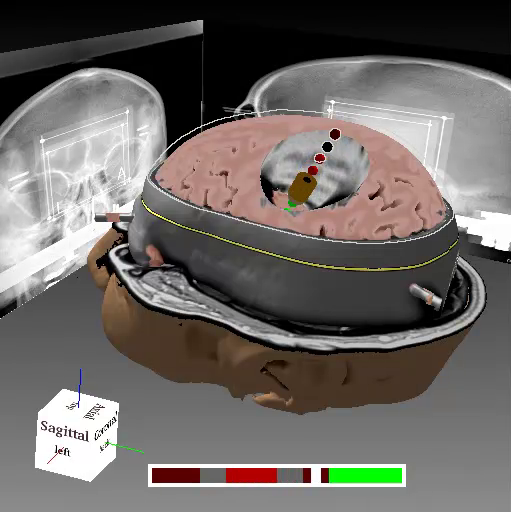
\includegraphics[width=0.495\linewidth]{verification-3d.png}
%\hspace*{0.5cm}
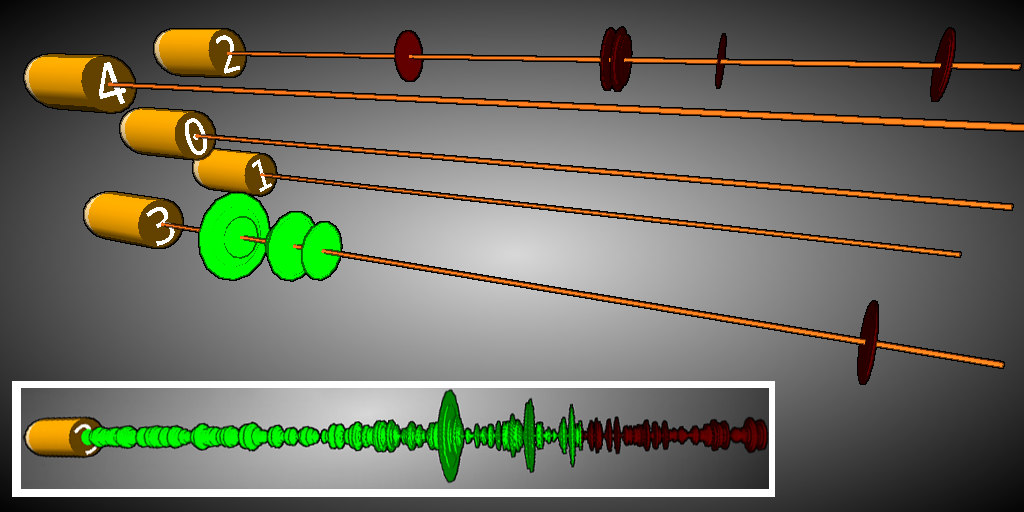
\includegraphics[width=0.495\linewidth, height=0.495\linewidth]{recording-3dsound.png}
\caption{View showing the imaging data combined with the analyzed MER recording data shown.}
\label{figure1}
\end{figure}


\section{Method}
Current systems require the surgeon to maintain a mental registration between the imaging modality and the electrical signals coming from the electrodes. By presenting the MER signal in a spatial context together with the imaging data we reduce the surgeon's cognitive load as he does not have to keep the spatial orientation of the electrodes or the previous analyses in mind.

Figure~\ref{figure1} shows two views from our system side-by-side. The left image shows the imaging data with an electrode tailed by colored beads representing the detected functional areas. The right image is a spatialized presentation of the electrical signals where peaks over a certain threshold are shown. While the left picture is an overview of all available data, the right picture shows the relative position of the electrodes with the time domain signal in the same spatial context. The cameras of both views are liked in order to retain the mental registration.

\section{Conclusion}
By collaborating closely with our partners from the St. Barbara Hospital in Hamm we were able to refine the system by constant feedback from domain experts. As a future work we will conduct a thorough user evaluation to assess the practibility of our system.

%\bibliographystyle{eg-alpha}
\bibliographystyle{eg-alpha-doi}
\bibliography{literature}

\end{document}
